\documentclass{report}
\usepackage{listings}
\usepackage{graphicx}
\usepackage{amsmath, amsthm,  amsfonts, amscd}
\usepackage{url}
\usepackage[a4paper, margin=3cm]{geometry}
\usepackage{algorithm}
\usepackage{algorithmic}
%\usepackage[]{algorithm2e}


\usepackage{afterpage}

\newcommand\blankpage{%
    \null
    \thispagestyle{empty}%
    \addtocounter{page}{-1}%
    \newpage}

%----- These are some of my macros by way of example ----------

\DeclareMathOperator{\sign}{sign}
\DeclareMathOperator{\mesh}{mesh}
\DeclareMathOperator{\vol}{vol}
\DeclareMathOperator{\Aut}{Aut}
\DeclareMathOperator{\End}{End}
\DeclareMathOperator{\tr}{tr}
\DeclareMathOperator{\Mod}{Mod}
\DeclareMathOperator{\Fred}{Fred}
\DeclareMathOperator{\CCh}{Ch}
\DeclareMathOperator{\coker}{coker}
\DeclareMathOperator{\Tr}{Tr}
\DeclareMathOperator{\Pro}{Pro}
\DeclareMathOperator{\Lin}{Lin}
\DeclareMathOperator{\Bun}{Bun}
\DeclareMathOperator{\ind}{ind}
\DeclareMathOperator{\hol}{hol}
\DeclareMathOperator{\Map}{Map}
\DeclareMathOperator{\E}{\mathbb{E}}
\newcommand\widebar[1]{\mathop{\overline{#1}}}


%-----------------------------------------------------------------------
% theorems, lemma etc
\theoremstyle{plain}
\newtheorem{theorem}{Theorem}[section]
\newtheorem{lemma}[theorem]{Lemma}
\newtheorem{proposition}[theorem]{Proposition}
\newtheorem{question}[theorem]{Question}

\theoremstyle{definition}
\newtheorem{definition}[theorem]{Definition}

\theoremstyle{remark}
\newtheorem{example}{Example}[section]
\newtheorem{note}{Note}[section]
\newtheorem{exercise}{Exercise}[section]


\numberwithin{equation}{section}
\numberwithin{figure}{section}

% ------------------------------------------------------------------------
% caligraphic
\newcommand{\cH}{{\mathcal H}}
\newcommand{\cS}{{\mathcal S}}
\newcommand{\cA}{{\mathcal A}}
\newcommand{\cE}{{\mathcal E}}
\newcommand{\cK}{{\mathcal K}}
\newcommand{\cU}{{\mathcal U}}
\newcommand{\cD}{{\mathcal D}}
\newcommand{\cP}{{\mathcal P}}

% math blackboard
\newcommand{\CC}{{\mathbb C}}
\newcommand{\RR}{{\mathbb R}}
\newcommand{\ZZ}{{\mathbb Z}}
\newcommand{\QQ}{{\mathbb Q}}

% greek
\renewcommand{\a}{\alpha}
\renewcommand{\b}{\beta}
\renewcommand{\c}{\gamma}

% miscellaneous


\newcommand{\<}{\langle}
\renewcommand{\>}{\rangle}

\newcommand{\cstar}{C^*}
\newcommand{\CCstar}{C^*}

%
%------ document begins -------------------------------------

%
\begin{document}


%
%-----beginning of title page -----------------------------
%
\begin{titlepage}
\begin{flushleft}
\hrule
\vspace{1 cm}


{\huge{\bf Learning to Generate Videos From Text}}
\vspace*{2cm}




\vspace{1 cm}
{\large Miguel Martin}

\vspace{0.5 cm}

{\large Supervisors: Dong Gong and Qinfeng Shi}

\vspace{0.5 cm}

{\today}

\vspace{2.5 cm}

    { Thesis submitted for Bachelor of Computer Science (Honours) }


\vspace{10 cm}


\hrule


\end{flushleft}
\begin{flushleft}
\textbf{\textsf{SCHOOL OF COMPUTER SCIENCE}}
\end{flushleft}


\vspace{-1cm}
%
% Adelaide University Crest
%

%
\begin{flushright}

\includegraphics[scale=0.25]{ua_crest.pdf}
\end{flushright}
\vspace{-2 cm}

\end{titlepage}


%
%---------- end of title page -------------------------------
%
\pagenumbering{roman}

\chapter*{Declaration}

Except where stated this thesis is, to the best of my knowledge, my own work and my supervisor has approved its submission.

\vspace{20 pt}

\begin{flushleft}
Signed by student:  \\[15 pt]
Date:
\end{flushleft}

\vspace{20 pt}
\begin{flushleft}
Signed by supervisor:\\[15 pt]
Date:
\end{flushleft}




%\chapter*{Acknowledgements}

\chapter*{Abstract}

The main topic of this thesis is learning to generate videos relating to a given text description. Learning is achieved through generative models in Machine Learning, specifically Generative Adversarial Networks.

\tableofcontents

\pagenumbering{arabic}
%
%---------------- thesis ------------------------------------
%
\chapter*{Introduction}
\addcontentsline{toc}{chapter}{Introduction}

%This is the introduction.  Here is a reference to somebodies paper  \cite{Hit}.

\section{Project Aims and Contributions}

The first aim is to cover the current state of the art in Machine Learning research relating to conditional and unconditional generative models for images and videos. The second aim will be take the concepts learned from the state of the art research and construct a new generative model that will aim to out-perform existing baseline models. Finally, the third aim will be discuss short-comings of the work performed, potential work for future improvements and other potential directions.

All code written during the thesis is freely available on Github \cite{martin_miguelmartin75/txt2vid_nodate}.

\section{The Problem At Hand}

Simply stated, we wish to learn to generate a video from a textual description. For instance, `a woman cuts some lettuce' should display some lettuce being chopped (as shown in Figure \ref{fig:example}). For simplicity, we will assume videos are of constant length (16 frames) and are up to 128x128 in resolution (with all smaller resolutions being a square aspect ratio).

\begin{figure}[H] \label{fig:example}
    \centering
    \caption{`a cat eats corn-on-the-cob' (top), `a woman cuts some lettuce' (bottom). Raw data MRVDC \cite{noauthor_microsoft_nodate}}
    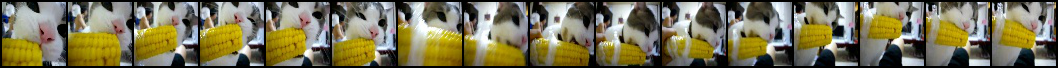
\includegraphics[width=0.8\linewidth]{images/cat_real.png}\\
    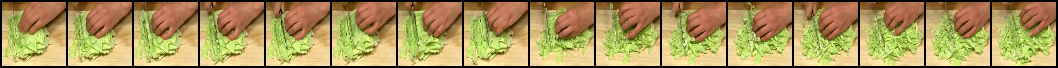
\includegraphics[width=0.8\linewidth]{images/real_131.png}\\
\end{figure}

\subsection{Attributes of a Solution}

There are multiple attributes we wish to consider whilst generating videos, the main ones this thesis will focus on is: 

\begin{enumerate}
    \item \textit{Visual quality}\\
        How good does the video look?
    \item \textit{Visual fidelity (feasibility)}\\
        Is the content within the video feasible and consistent given the context of the videos being generated, e.g. if the video contains a man, does the figure look like a human-being?
    \item \textit{Motion}\\
        If we are generating static videos, then this is no different to generating images.
    \item \textit{Correlation to the input sentence}\\
        Does the video actually correlate to the input sentence?
    \item \textit{Diversity}\\
        Are we generating the same video over and over? 
    \item \textit{Generalisation}\\
        If we give our generator a sentence it has not seen before, does it a coherent video videos (adhering to the above properties)?
\end{enumerate}

There are numerous other factors, as mentioned in my proposal. However, for simplicity's sake these properties will be focused on.

\section{Thesis Outline}

Chapter 1 will discuss a brief background to various underlying Machine Learning concepts related to generative modelling, mostly related to Generative Adversarial Networks (GANs).\\

\noindent
Chapter 2 will discuss related work and state of the art research done related to video classification, and video/image generation.\\

\noindent
Chapter 3 will discuss my proposed solution with Generateive Adversial Networks (GANs), and how I decided to model based off existing work in the field.\\

\noindent
Chapter 4 will cover the experiments I performed throughout the development of my project.\\

\noindent
Finally, Chapter 5 will conclude my thesis and discuss potential future work and improvements that can be made.

\newpage

\blankpage
\chapter{Background}

This section contains some definitions and background research relevant to the material of the thesis.

\section{Machine Learning}
Machine Learning can be loosely defined as: given a set of data, we wish to find some underlying process for which models this data for some potential task. More concretely, let us assume our set of data is $\vec{x}$, this underlying process is $f$, we wish to find some $g$ where $f(\vec{x}) \approx g(\vec{x})$.

Common tasks in Machine Learning include classification and clustering. Typically a sample or example within the set of data is defined as a set of features (represented by a vector), where each feature is represented by a discrete or continuous variable.

\section{Supervised Learning}
Supervised learning, the most common form of learning, is where we have access to the associated values of the underlying process of the task (commonly referred to as labels, classes, outputs, etc.), i.e. we have a pair of values $(\vec{x}, f(\vec{x}))$, for every possible sample data-point $\vec{x}$ in our dataset. Common uses of supervised learning are for classification or regression tasks, where $f(\vec{x})$ is discrete or continuous respectively.

\section{Unsupervised Learning}
Unsupervised learning can is simply where we only have access to our data-points and not associated values for the underlying process, i.e. we do not have $f(\vec{x})$. Common tasks for unsupervised learning include clustering and generative modelling. Unsupervised learning techniques are especially useful when used in conjunction with transfer learning (see below), as they allow for pre-training without additional data and allow us to start at a better prior (compared to random initialisation). 

\section{Auto-Encoders}
An auto-encoder \cite{goodfellow_deep_2016} is an unsupervised leaning method that aims to learn some representation for some given input sample with two neural networks: an encoder and decoder network. This representation is typically lower dimensional than the input feature size, in order to force one to learn a meaningful representation. In other words, we wish to learn two functions $f$ and $g$ where $f(g(x)) \approx x$, where $f$ is our decoder and $g$ is our encoder network. This technique will be utilised for the training of the generative model produced.

\section{Generative Modelling}

Generative modelling can be viewed as an unsupervised learning problem, where we have some generative model which attempts to capture/understand the \textit{underlying} distribution of the input data for generative purposes.

\section{GANs}
Generative adversarial networks \cite{goodfellow_generative_2014} model the generative problem as a two player game with two neural networks competing against each other. One network attempts to generates fake samples (the generator) and the other network attempts to differentiate (classify) the difference between real samples and generated samples (the discriminator). The game is simple, the generator aims to fool the discriminator whilst the discriminator learns to distinguish between real and fake samples. We require to find a Nash equilibrium of the min-max problem (defined in equation \eqref{eq:gan}). 

\begin{equation}
\label{eq:gan}
    \min_{G} \max_{D} \E_{x \sim q_{\text{data}(x)}}[log D(\vec{x})] + \E_{z \sim p(\vec{z})} [ log(1 - D(G(\vec{z}))) ]
\end{equation}

As suggested in the above equation, the generator network learns to map data from some prior distribution to the underlying data distribution. This `latent' variable is typically a multi-dimensional vector, and is from some known prior distribution, such as the normal distribution

To optimise this problem we can use gradient descent, the original GAN paper uses SGD with momentum \cite{goodfellow_generative_2014}, but other variations use Adam (\cite{radford_unsupervised_2015, gulrajani_improved_2017}). Specifically the (generalised) GAN algorithm can be described as follows:

\begin{algorithm}
\label{ganalgo}
    \caption{A generalisation of the GAN algorithm. $n_D$ is the number of discriminator steps ($n_D = 1$), $n_G$ is the number of generator steps ($n_G = 1$), $\theta$ are the parameters for the generator and $\omega$ are the parameters for the discriminator} 

\begin{algorithmic}
    \FOR{number of training iterations}
    \STATE{
        \FOR{t = 1, ..., $n_D$}
        \STATE{
            \STATE Sample a mini-batch of m-noise samples $\{ \vec{z}^{(1)}, ..., \vec{z}^{(m)} \}$ from a prior distribution $p(\vec{z})$\\
            \STATE Update the discriminator by ascending its stochastic gradient, where the gradient is defined by:
                \[
                    \nabla_{\theta} \frac{1}{m} \sum_{i-1}^{m} [ log(D(x^{(i)}) + log(1 - D(G(z^{(i)}))) ]
                \]
        }
        \ENDFOR
        \FOR{t = 1, ..., $n_D$}
        \STATE{
            \STATE Sample a mini-batch of m-noise samples $\{ \vec{z}^(1), ..., \vec{z}^(m) \}$ from a prior distribution $p(\vec{z})$\\
            \STATE Update the generator by descending its stoshastic gradient, where the gradient is defined by:
            \[
                \nabla_{\theta} \frac{1}{m} \sum_{i=1}^{m} [ log(1 - D(G(z^{(i)}))) ]
            \]

        }
        \ENDFOR
    }
    \ENDFOR
\end{algorithmic}

\end{algorithm}

GANs have various issues as noted in the original paper \cite{goodfellow_generative_2014} and other papers \cite{gulrajani_improved_2017,arjovsky_wasserstein_2017,jolicoeur-martineau_relativistic_2018}. These issues include:

\begin{enumerate}
    \item \textit{Training instability}\\
        Unlike typical optimisation problem where we purely minimise (or maximise) some objective, we want our generator and discriminator networks to be approximately equal. This is so that our our generator can progress and produce better samples. Intuitively, if either the discriminator or generator becomes too strong (relatively), then at this . 
    \item \textit{Hyper-parameter sensitivity}\\
        This issue ties in with the previous. The choice of hyper-parameters is more of an art right now. The choice of the learning rate, architectures, etc. are very important. If something is off then it will be evident in the samples produced by the generator.
    \item \textit{Mode collapse}\\
        This is simply when the generator learns to produce the same outputs. It is a pretty common issue.
    \item \textit{Generalisation issues}\\
        Generalisation, in the context of generalisation, is the concept of generating something that was not there. It is common for GANs to not have good generalisation.
    \item \textit{Time to Train}\\
        GANs typically take a long time to train, as they require to do many iterations, which is more of an annoyance than anything else.
\end{enumerate}

There have been attempts to alleviate these issues, which are discussed in the `Related Work' section.

\subsection{Conditional GANs}
A conditional GAN is a modification of the standard GAN which aims to generate samples that are conditioned on some conditioning information. There are multiple ways to include conditional information into the GAN architecture. The simplest approach is to simply concatenate the features of the conditioning information with the latent variable. From there there are a couple of approaches to train the conditional GAN. The simplest approach is to treat this as a regular GAN and simply train it as-is \cite{mirza_conditional_2014}. Instead of applying the regular GAN algorithm, we can modify the loss for the generator and discriminator.

An alternative is to interpret the discriminator as classifying whether a sample and conditioning input pair are associated. Then we can simply ask the discriminator to check three pairs: $(x_r, c_r)$ [should be associated], $(x_f, c_r)$ [should not be] and $(x_r, c_f)$ [should not be]; where $x_r$ represents a real sample, $x_f$ represents a fake sample, $c_r$ represents associated conditioning information and $c_f$ represented un-associated conditioning information. The final pair $(x_f, c_f)$ is not used, as this pair does not provide much information; intuitively at least, to my knowledge no experimentation of this has been performed. It is unclear which approach is better, but this approach is utilised in many conditional GANs \cite{pan_create_2018,zhang_stackgan++:_2017}.


\section{Transfer Learning}
\textit{Transfer learning} is a simple, yet very effective, training technique. A pre-trained neural network that solves one particular task and/or dataset distribution and use those parameters to train another neural network (of similar or the same architecture) for another task and/or dataset distribution. Transfer learning is extremely useful if the task we want to solve has little amounts of data.

\blankpage
\chapter{Related Work}

\section{Video Classification}

Video classification (the inverse of our problem) is of interest due to two reasons: firstly, a powerful video classification model can also enable us to evaluate our generative model, e.g. with FID \cite{heusel_gans_2017} or an Inception Score \cite{salimans_improved_2016}. Secondly, a GAN's discriminator network can be viewed as classification model. Thus looking into research related to video classification may be necessary to determine what a powerful discriminator function could potentially look like.

\subsection{Inflated Convolutions}

An inflated convolution, introduced by Carreira et al. \cite{carreira_quo_2017}, is a simple technique to transform an existing 2D convolutional network architecture (CNN) and expand it to a 3D convolutional network for video input. All kernels for pooling and convolutional layers are inflated by simply making square $N \times N$ kernels into cubic $N \times N \times N$ kernels (most kernels are square). Note that for some pooling layers, Carrerira et al. \cite{carreira_quo_2017} found it is better to not perform temporal pooling, i.e. $N \times N$ pooling layers are converted to $1 \times N \times N$.

Carreira et al. \cite{carreira_quo_2017} also introduce a simple (but creative) technique to utilise pre-trained weights for a 2D CNN (say from ImageNet) and use them for an inflated 3D CNN, dubbed `bootstrapping'. Simply put, for a 2D convolutional kernel inflated to a 3D kernel, they repeat the weights and divide the weights by a factor of $N$. They do this to allow for `boring' videos, where an image is stacked along the time dimension to create a static video, to enforce the 3D inflated network to produce the same output as the corresponding 2D CNN. 

Inflated convolutional neural networks, when bootstrapped, out-perform many different architectures; including an LSTM and non-bootstrapped inflated networks on multiple datasets as noted by \cite{carreira_quo_2017}.

\subsubsection{Two-Stream Network (I3D)}

Carreira et at. \cite{carreira_quo_2017} also experimented with inflated networks for classification tasks with additional pre-computed features for motion, they label this model as `I3D'. These motion features are simply optical flow (pre-computed). I3D (with two-stream) out-performs the equivalent network by 3.1\% (top-1 test) to 3.7\% (top-1 validation) \cite{wang_non-local_2017} on the Kinetics dataset \cite{kay_kinetics_2017}, signifying the importance of motion. These results also suggest that 3D convolutions on their own is not sufficient to capture a good features from the temporal dimensions related to motion.

\subsection{Non-Local Blocks}

Wang et al. \cite{wang_non-local_2017} introduced the concept of non-local operations for deep neural networks, which directly responds to the work done by Carreria et al. \cite{carreira_quo_2017}. A non-local operation is a 1-to-1 operation, which computes a weighted sum for some learnt relationship (function) between \textit{all possible} positions. These set of positions could be time, space or spacetime, e.g. spacetime for video. It should be noted that non-local operations are different to
fully-connected layers, as the relationship between two positions is a learnt function rather than a simple scalar weight. This is demonstrated in the equation for a non-local operation (equation \eqref{eq:non_local}).

\begin{equation}
\label{eq:non_local}
    y_i = \frac{1}{C(x)} \sum_{\forall j} f(x_i, x_j) g(x_j)
\end{equation}

where $i$ is the index of the output position, $C(x)$ is some normalising factor, $f$ is some (learnable) function that determines the relationship between two positions and finally $g$ represents some function to output the weight for two positions.

A non-local block simply refers to a wrapping of a non-local operation in a residual block \cite{he_deep_2015}, i.e. for the $i$th layer $\vec{x}_i' = w_i \vec{y}_i + \vec{x}_i$ where $\vec{x}_i$ denotes the output of the $i$th layer in the original network, $w_i$ some scalar weight and $\vec{y}_i$ is the output given by the non-local operation (equation \eqref{eq:non_local}). Non-local blocks are useful as they allow non-local operations to be incorporated in existing architectures without changing the potential behaviour of the network (if $w_i$ is zero then we have the original network). Thus transfer learning can be trivially accomplished by assigning $w_i$ to zero.

Non-local operations allow to capture the global structure of the feature space. The alternative to non-local operations in existing architectures would be deeper networks. For convolutional networks, this would require stacking various convolutional layers, which is done extensively in existing state of the art architectures for image classification. Thus, without non-local operations, long range dependencies would require deeper networks and therefore require more parameters to train.

Non-local operations are a good alternative to alleviate this, as the number of additional parameters required is not very significant for the performance benefits. However, contrary to convolutional layers, as found by \cite{wang_non-local_2017} adding more non-local blocks in a network does not simply allow for significant performance gains. Intuitively this makes sense, due to a non-local operation considering all pairs of features (all possible positions) at any place it is performed in the network. For a ResNet-101 \cite{he_deep_2015} (a 101 layer convolutional network), they found no difference in test error with 5 and 10 non-local blocks and the difference between 1 and 5 non-local blocks is relatively small (around 1\% for both ResNet-50 and ResNet-101).

Placing non-local blocks after convolutional layers with smaller kernel sizes was found to be most effective, potentially due to positional information being more precise, as hypothesised by \cite{wang_non-local_2017}. $f$ as a Gaussian ($f = e^{\vec{x}_i^T \vec{x}_j}$) and $g$ as a linear embedding was found to be most effective. For video, spacetime non-local operations are most effective. Finally, a non-local I3D (without two-stream) out-performed the equivalent I3D (with flow) by around 1\% \cite{wang_non-local_2017}. This suggests non-local blocks are more than capable of learning motion, and the motion features they do learn is more effective than optical flow as features.
 
\section{Generating Images}

\subsection{StackGAN++}

StackGAN++ \cite{zhang_stackgan++:_2017} provides a basic architecture for stacking multiple GANs together to solve the task of image generation conditioned on text. The basic idea behind this architecture is to have multiple generators and discriminators, stacked together in a tree-like structure. Each generator depends on the previous generator's feature map (note: not rendered image) and each generator progressively increases the resolution of the generated image. Each disriminator simply discriminates the 

Additionally, StackGAN++ \cite{zhang_stackgan++:_2017}, can learns the conditional and unconditional image distributions jointly. By making the discriminator have two outputs; this requires the conditioning information to be concatenated with some feature space of the input data at the end of the discriminator network. With this, we can then simply take the average of the conditional and unconditional loss.

\subsection{BigGAN}
BigGAN \cite{brock_large_2018} proposes the first GAN architecture to generate very realistic images of high resolution that does not progressively grow in size or consists of stacking multiple generative models. Note that they provide models for both class-conditional and unconditional variations of the image generation problem. The architecture they use is based on Self-Attention GAN \cite{zhang_self-attention_2018}, which utilise non-local blocks \cite{wang_non-local_2017} in both the discriminator and generator. They achieve their performance boosts by a wide variety of techniques, most notably:

\begin{enumerate}
    \item Larger batch size generally equates to better video generation.
    \item Increase the width of the discriminator and generator (number of channels) by 50\%, this increases performance by 21\% (relative to the inception score). They note that increasing depth did not initially improve performance, but they address this in their deeper model by modifying the architecture.
    \item Skip-z connections. These are simple skip connections from the latent variable ($z$) to multiple layers in the generator. This improves training speed by around 18\% and a general improvement of 4\%
\end{enumerate}

BigGAN also utilises hinge loss, orthogonal initialisation and regularisation \cite{brock_large_2018}. 

\section{Generating Videos}

\subsection{Video Generation From Text}
`Video Generation From Text' \cite{li_video_2017} introduces a hybrid approach to generate videos from text, with a conditional Variational Auto Encoder (c-VAE) and a DCGAN \cite{radford_unsupervised_2015}. This DCGAN utilises 3D de-convolutional layers in the generator and 3D convolutional layers in the discriminator \cite{li_video_2017}. Text is encoded with an RNN, specifically a bi-directional LSTM to a fixed length feature vector, via using the last hidden state. The WGAN algorithm is utilised for learning \cite{arjovsky_wasserstein_2017}. 

Their c-VAE is conditioned on the encoded text and first frame of the video (encoded with a CNN) during the training process (and unconditioned during evaluation), first predicts a `gist'. This gist aims to simultaneously capture the layout/structure of objects within the video and the background colour/general aesthetics of the video \cite{li_video_2017}. 

Videos are generated through their DCGAN, which is conditioned on the `gist' and text. In order to combine these two variables, ‘Text2Filter’ is utilised. `Text2Filter' is simply a convolutional layer, where the input text feature vector is replicated across the gist image and concatenated with the `gist' along the channel dimension. The convolutional layer is utilised over a simple concatenation, as it was noticed that the model would give too much emphasis to the text or gist image. The discriminator also uses ‘Text2Filter’, but with the input video instead of the gist.

The data used is a set of (very) simple sentence (e.g. `a man plays golf') describing an action for a short video clips from the Kinetics Human Action Video Dataset \cite{kay_kinetics_2017}. Finally, they conclude that their approach out-performs other simpler approaches, namely their model without the inclusion of the ‘gist’ and Text2Filter (both combinations of the two). As videos are associated with actions, they use an Inception score for quantitative comparisons, with a separate model predict predicting the associated action for an output video.

\subsection{To Create What You Tell: Generating Videos from Captions}
`To Create What You Tell' \cite{pan_create_2018} (TCWYT) and `Video Generating from Text' \cite{li_video_2017} both have many similarities. They both utilise GANs, but TCWYT does not utilise a VAE or predict a ‘gist’ or background prior to generating the video. Instead, they propose the utilisation of three discriminators to ensure the generator produces:

\begin{enumerate}
    \item A discriminator that determines if video and sentence pairings are correlated
    \item A discriminator that determines if individual and sentence pairings are correlated. From a theoretical perspective this is equivalent to the above, but they notice that from an empirical perspective the model out-performs without it.
    \item A discriminator to determine if motion (temporal coherence) is correctly associated with the given sentence.
\end{enumerate}

Motion is simply described as the difference between two frame. Specifically the difference between the features of each frame (as predicted by the above model). They propose an alternative to this and that is to minimise the difference of two frames via L2 norm, but they hypothesis and show empirically that adversarially learning this is significantly better. To give the discriminators the input of a 3D or 2D matrix concatenated with text for conditioning purposes, they also perform something equivalent to ‘Text2Filter' as described in the previous paper. The ‘Text2Filter' only after to the text vector being transformed with a fully connected layout first.

The data they use is YouTube cooking clips from the Microsoft Research Video Description Corpus (MRVDC) dataset \cite{noauthor_microsoft_nodate}. A Generative Adversarial Metric (GAM) is utilised for a quantitative measure. This metric puts two generative adversarial models against each other in battle. It utilises the ratio of correct classifications from a test distribution, and also compares the number of times a discriminator is fooled by the opponents generator. The winner is defined by a simple heuristic which favours the ability to fool the opponent assuming the classification accuracy is approximately the same. They produce reasonable results, one might argue slightly better than the previous paper.

\subsection{TGAN and TGANv2}

TGAN \cite{saito_temporal_2016} and TGANv2 \cite{saito_tganv2:_2018} re-model the problem slightly. Instead of the generator producing a video at once, e.g. with 3D de-convolutional layers, generation is instead done by producing videos at a frame-by-frame level, i.e. the generator is an image generator. To do this, both TGAN and TGANv2 produce a set of latent variables to be used as input to the generator from one latent variable, e.g. from a 256 latent variable sampled from the normal distribution, they produce $16\times256$ latent variable. TGAN does this via a 1D de-convoltional network and TGANv2 does this with a Convolutional LSTM (CLSTM) \cite{shi_convolutional_2015}. TGANv2 provides an interesting concept labelled `subsampling layers', which is utilised to reduce memory consumption.

Simply put, a sub-sampling layer (with adaptive batch reduction) reduces the batch size and temporal dimension by some constant factor of the given input (e.g. by a factor of 2). In other words, it takes some input of size $B \times C \times T \times H \times W$ and reduces this to $\lceil \frac{B}{2} \rceil \times C \times \lceil \frac{T}{2} \rceil \times H \times W$, note that if $T=1$ or $B=1$ they are left unchanged. One can implement it as follows (in python, using numpy slicing syntax) \texttt{x = x[::bn, :, bt::st]}, where $b_t \sim \text{unif}(0, s_t - 1)$, $s_t$ and $b_n$ are constants ($s_t = b_n = 2$). In other words, this takes every $b_n$th sample for the batch dimension and every $s_t$th frame, starting at $b_t$.

TGANv2's approach to video generation is similar to that of StackGAN++ \cite{zhang_stackgan++:_2017}, as it generates videos at multiple scales. Their generator is composed of multiple sub-generators, which are all are stacked akin to StackGAN++. These sub-generators have associated `render blocks', which produce videos at various resolutions; multiple discriminators for each resolution. Their model is composed of $L$ sub-generators with $L - 1$ sub-sampling layers (with adaptive batch reduction, which are applied after the first sub-generator), $L = 4$ for all experimented TGANv2 models. During evaluation/inference, subsampling layers are disabled in order to allow for the network to generate a full video in the largest possible resolution.

\section{Relativistic Discriminator}

The relativistic discriminator \cite{jolicoeur-martineau_relativistic_2018} transforms a discriminator (from a GAN) to judge real and fakes in a relative manner. It does this modifying the loss of the discriminator, see equation \eqref{eq:rel_loss_discrim} and \eqref{eq:rel_loss_gen}. Abstractly the modifications performed can be thought as transforming the traditional question a discriminator answers: `what is the probability that this sample is in the underlying real data distribution?' to `what is the probability of the real sample being more realistic than the fake sample?'.

\begin{equation}
    \label{eq:rel_loss_discrim}
    L_{D} = -\E{[\text{log}(\text{sigmoid}({D_i(\vec{x}) - D_i(G(\vec{z}))})]}
\end{equation}

\begin{equation}
    \label{eq:rel_loss_gen}
    L_{G} = -\E{[\text{log}(\text{sigmoid}({D_i(\vec{x}) - D_i(G(\vec{z}))})]}
\end{equation}

It is also extended for other loss functions in a similar manner. Most notably the above loss, dubbed relativistic standard GAN (RSGAN) loss, with gradient penalty gave the best convergence results (in terms of FID and Inception Score) with one step of the discriminator per one step of the generator. Thus this loss is experimented with.

\blankpage
\chapter{Proposed Solution}

The main focus of the thesis is Generative Adversarial Networks (GANs), as such this section will discuss each component of a proposed GAN. This section includes the training procedure, the architectures (and design decisions) for the language model (conditioning information), the discriminator and generator.

\section{Why GANs?}

Generative Adversarial Networks (GANs) were chosen to be the generative model of choice. This is due to the following factors:

\begin{enumerate}
    \item \textit{Existing Work}\\
        GANs achieve state of the results in many generative tasks, including images \cite{zhang_stackgan++:_2017}, unconditional videos \cite{brock_large_2018}, and the problem we are tasked to solve itself \cite{pan_create_2018} (conditional videos).
    \item \textit{Simplicity}\\
        Adversarial training is quite powerful due to is simplicity. It can be quite easily understood, which is vital for research.
    \item \textit{Memory Constraints}\\
        Simple techniques can be used to reduce the memory requirements to allow for larger resolution videos to be generated. Other architectures, namely invertible networks \cite{kingma_glow:_2018} will require more memory (to produce an equivalent video) due to the network requiring to be to be 1-to-1 function (the input size must equal the output size).
\end{enumerate}

GANs do have their drawbacks, which were notable throughout the project (as mentioned in Background) which were present throughout the development of the project. This is even with improvements such as WGAN-GP \cite{gulrajani_improved_2017}.

In my research proposal, invertible/reversible networks \cite{jacobsen_i-revnet:_2018,kingma_glow:_2018} were chosen as the generative model to be looked into, as I believed they would allow for advancements in the field. However, due to a lack of proper understanding (hence making it hard to perform research) and their complexity over GANs, they were dropped. The biggest issue invertible networks suffer from is memory usage, to put this into context, GLOW \cite{kingma_glow:_2018} has about 200 million parameters for 256x256 images.  Since 1x1 convolutions are used, a naive extension to GLOW would require a factor of $O(T)$ more parameters (where $T$ is the number of frames in the video). Perhaps a (very) small batch size and/or half-precision (or mixed-precision) training could be utilised to mitigate this issue.

Still, invertible/reversible networks are an interesting topic, and may be of interest for future work. If one wanted to direct their research into reversible networks, then I believe the feasibility of the unconditional task should be first evaluated.

\section{Baselines}

There are two baseline models for which we will make all comparisons and extensions to. The first is the conditional model introduced in `To Create What You Tell Model' (TCWYT) \cite{pan_create_2018}. This baseline was chosen because the work performed in this paper models precisely what we aim to accomplish; that is generating video by conditioning on text. Thus, we aim to iterate upon their work.

The second is the unconditional model found in TGANv2 \cite{saito_tganv2:_2018}, the architecture and training procedure heavily influenced what was built upon. Comparisons to this model are made for two reasons. Firstly, to ensure the validity of my implementation as code for this TGANv2 is not released. Secondly, this model has many more parameters than the conditional baseline, and as such it would be an unfair comparison.

\section{The Language Model}

A small bi-directional LSTM model will be used to encode textual information, similar to what is performed in TCWYT \cite{pan_create_2018}. This bi-directional LSTM has 4 layers and a hidden state size of 256, words are embedded prior to feeding them through the network. The final hidden state of the last layer in the network is used as an encoding of the input text.

Similar to \cite{pan_create_2018} pre-training consists of simply using the language model similar to an auto-encoder. That is, feed the text through the network with an aim to re-produce the same sentence from the hidden states. This pre-training method was introduced in \cite{dai_semi-supervised_2015}, it is very effective for transfer learning purposes, with many tasks benefiting from it significantly.

Utilising GPT-2 \cite{radford_language_2019} would be an interesting extension to the language model and was considered. However, there is a major limitation with this approach, which is related to the model size. GPT-2 is a large model ($1.17*10^8$ parameters in the smallest model), and as such will take longer to train and require more memory; hence it may restrict us by using a smaller batch size (which is not good \cite{brock_large_2018}) or take away from the parameters of the discriminator or generator. However, one could nullify this limitation by not training the network end to end, by either using zero-shot learning or simply fine-tuning the model for the target text domain (e.g. via the pre-training method as mentioned above). It is not clear whether the textual encoder is a major bottleneck when. The assumption that it is not a major bottleneck is made, and focus is made on experimenting with the generator/discriminator.

\section{Architecture}

The general architecture and training procedure is heavily influenced by TGANv2 \cite{saito_tganv2:_2018}, specifically the architecture for the generator and discriminator mainly remains the same. Modifications are made to the architecture and training procedure, due to TGANv2 not being a conditional model \cite{saito_tganv2:_2018}. Architecture changes are inspired from Self-Attention GAN \cite{zhang_self-attention_2018} and BigGAN \cite{brock_large_2018}. StackGAN++ \cite{zhang_stackgan++:_2017}, TCWYT \cite{pan_create_2018}, and `Video Generation from Text' \cite{li_video_2017} all heavily influenced changes with respect to incorporating conditioning information to the model.

\subsection{Why take inspiration from TGANv2?}

The main inspiration from TGANv2 \cite{saito_tganv2:_2018} stems from it's creative sub-sampling layer with adaptive batch reduction, and impressive results in generating large videos. All other video generators generate videos of 64x64 or lower resolution \cite{pan_create_2018,li_video_2017}. When compared to TCWYT \cite{pan_create_2018}, it is obvious that TGANv2 \cite{saito_tganv2:_2018} has the potential to out-perform TCWYT \cite{pan_create_2018} by quite a large margin.

\subsection{Differences from TGANv2}

Modifications to the model presented in TGANv2 \cite{saito_tganv2:_2018} are done for two reasons, (1) to add conditioning information and (2) to take the additional lessons learned from BigGAN \cite{brock_large_2018} and apply them.

\subsubsection{Effectively Capturing Motion}

Non-local blocks \cite{wang_non-local_2017} are added to the generator and discriminator for motion and global structure. They are used in a similar manner to BigGAN \cite{brock_large_2018} and Self-Attention GAN \cite{zhang_self-attention_2018}. As discussed in Related Work, non-local blocks when applied after 2D or 3D convolutions provide many potential benefits for the little added cost in parameters. Most notably when spacetime non-local blocks are applied in conjunction with 3D convolutions (as used in the discriminator), we should be able to capture motion effectively (as mentioned in Related Work). In the following, we will discuss some alternatives:

The first option, is to simply let (and hope) the 3D convolutions capture motion, which is what TGANv2 does. However, as discussed above, utilising non-local blocks in conjunction with 3D convolutions increases the predictive power of the model for a not very high cost. This approach is decent, but it does not seem to be potentially as effective as it could be; hence the choice in adding non-local blocks.

The second option would be to either use the technique introduced in I3D \cite{carreira_quo_2017}, which requires pre-computed optical flow to be given in two-stream neural network (classifying on video features and pre-computed optical flow). Once again, this has been shown to be less effective than non-local blocks (as demonstrated in \cite{wang_non-local_2017}), when considering classification tasks, which effectively is what the discriminator is performing. 

Finally, another alternative would be to introduce a new discriminator that works at a per-frame level. Specifically this new discriminator could look at a pair of consecutive frames or the difference between two frames (as done in \cite{pan_create_2018}). This obviously would require significantly more parameters, especially if we (1) scale this discriminator to be of the same margin in parameters as the main (multi-scale) discriminator and/or (2) use multiple instances of this discriminator for the different scales of video the generator produces during training.

Similar to BigGAN \cite{brock_large_2018} for their 128x128 models: a single non-local block is added to the generator after the second to last up block, and a single non-local block is added after the first down block in the discriminator.

\subsubsection{Adding Conditional Information}

We learn conditioning information jointly, similar to StackGAN++ \cite{zhang_stackgan++:_2017}. We also utilise a relativistic discriminator, and as such we must modify the relativistic loss to handle conditional information. Specifically we base our loss of the Standard GAN Loss, as it seems to be most effective for a 1 discriminator to 1 generator step \cite{jolicoeur-martineau_relativistic_2018}. We relatively compare the pairs $\{(x_r, c_r)$, $(x_f, c_r)\}$ and $\{(x_r, c_f),(x_f, c_r)\}$, thus our conditional loss for the $i$th discriminator is:

\[
    L_{D_{i}}^{\text{conditional}} = -\frac{1}{2} \E{[\text{log}(\text{sigmoid}({D_i(x, c) - D_i(G(z, c), c)}))]} - \frac{1}{2} \E{[\text{log}(\text{sigmoid}({D_i(x, c) - D_i(G(z, c), \widebar{c})))]}}
\]\\

For the generator we only compare the pairs $\{(x_r, c_r)$, $(x_f, c_r)\}$, thus our generator (unconditional loss) is:

\[
    L_{G}^{\text{conditional}} = -\sum_{i=1}^{L}\E{[\text{log}(\text{sigmoid}({D_i(G(z, c), c) - D_i(x, c)}))]}
\]\\

As we learn the conditional and unconditional loss jointly, we simply average the conditional and unconditional loss.

\blankpage
\chapter{Experimentation}

\section{Datasets}

There are two datasets experimentation is performed on. The first is a toy moving MNIST dataset, synthetically generated from the MNIST dataset, sentences are made synthetically to describe a motion, for instance `the digit 9 is moving up and down'. This dataset setup is inspired from \cite{pan_create_2018}. This dataset was primarily used to see if my implementation was valid, it also shows some caveats with the current approach even in a perfect setting.

The second dataset is the cooking videos from the MSR Video to Text (MSRVDC) dataset \cite{noauthor_microsoft_nodate}, as utilised in TCWYT \cite{pan_create_2018}.

A third dataset was experimented on, which was a custom dataset collected, labelled `reddit videos'. Taking inspiration from GPT-2 \cite{radford_language_2019}, where the gifs sub-reddit was scraped, taking the titles as the caption for the video and utilising only posts with at least 5 upvotes. Unfortunately with the current implementation and model, it was impossible to converge to a solution, thus it will be excluded from this section.

\begin{figure}[H]
    \centering
    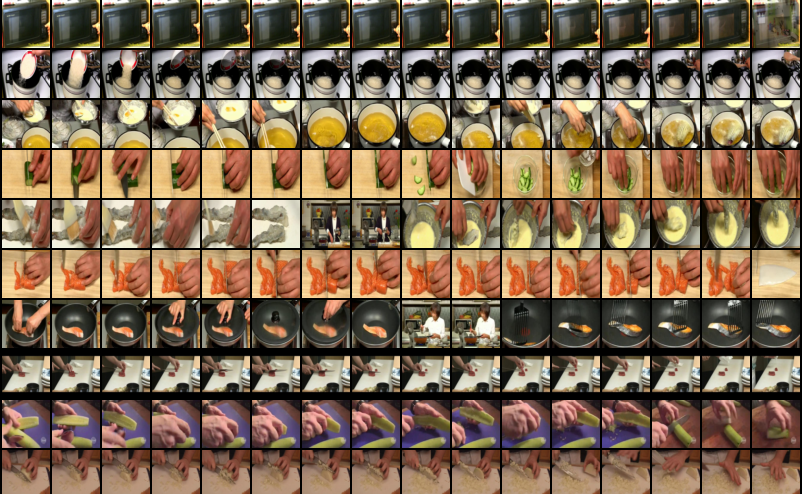
\includegraphics[width=0.8\linewidth]{../progress/imgs/mrvdc/real_samples.png}
    \caption{Some example real videos from the dataset}
\end{figure}

\section{Setup}

The baseline models and proposed models are trained on each dataset. I utilised Adelaide University's Phoenix HPC and my local setup (a 6GB GTX 1060), using both K80s and V100s whenever possible. The unconditional TGANv2 models were trained on 2 V100s with a batch size of 128 with a resolution of $128\times128$, with 4 generators and 3 sub-sampling layers with the same parameters as TGANv2; this model was trained for 28,000 iterations. The conditional TGANv2 model (what I proposed) was trained
on my GTX1060 with a resolution of $64\times64$ and a batch size of 40, as the V100s were inaccessible at the time and was trained for 10,000 iterations. For all models, the Adam optimiser was used with 1 discriminator step per generator step, with a $\text{lr} = 0.0002$, $b_1 = 0.5$, $b_2 = 0.999$. K80s were not used for the conditional model due to some odd bug or issue (e.g. with the implementation of cuDNN on the different architectures), this was regardless of the parameters I used (even if they were the same), a further discussion is mentioned below.

\section{Evaluation}

Subjective comparisons for generative models are quite common, and when done in a survey, can allow for a fair comparison. However, this is not ideal, due to cost and/or time. Instead, quantitative metrics can be utilised. These may not be as reliable as human surveys, but they can provide a deterministic metric. Ideally we would like a qualitative method that looks at visual quality, motion and sentence correlation in one or multiple metric. A FID score on a pre-trained I3D (or non-local network) was going to be utilised, but unfortunately was not incorporated.

This experimental setup will be using subjective measures (my eyes). This is mainly due to obvious nature of the current results.

\section{Results, Findings and Analysis}

\subsection{MNIST moving}

\subsubsection{TCWYT Baseline}

The main issues with the TCWYT baseline model for the MNIST dataset are:
\begin{enumerate}
    \item Occasional training artifacts (figure \ref{fig:artifacts_base}) in some iterations of the training process for some associated frames. I hypothesise this is due to my activation functions obtaining a negative slope, but since LeakyReLU was utilised this issue resolved itself with further iterations.
    \item Mode collapse as shown with Figure 3. This is likely due to there only being 36 possible combinations of the sentences, and thus it was likely learnt to simply generate from the sentence itself (i.e. the latent variable was ignored). This hypothesis is supported with the other dataset I tested with.
    \item Issues in the produced videos, i.e. moving in the wrong direction, morphing of digits (see Figure \ref{fig:wrongdir_base}). Likely due to the discriminators not performing correct classification (i.e. confusion with some digits). It is not clear how to resolve this issue.
\end{enumerate}

\begin{figure}[H] \label{fig:artifacts_base}
    \centering
    \caption{Occasional artifacts from training}
    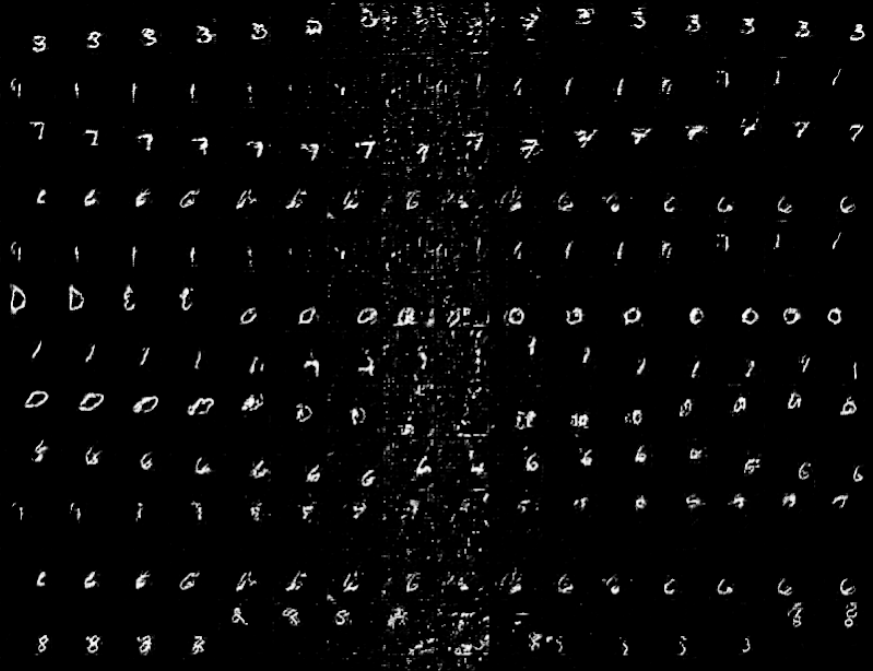
\includegraphics[width=0.8\linewidth]{../progress/imgs/mnist/mnist_artifacts.png}
\end{figure}

\begin{figure}[H] \label{fig:modecollapse_base}
    \centering
    \caption{Three generated samples with the same sentence but different latent variables (evidence of mode collapse)}
    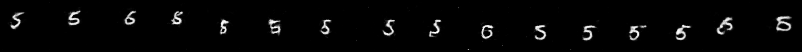
\includegraphics[width=0.8\linewidth]{../progress/imgs/mnist/mode_collapse.png}\\
    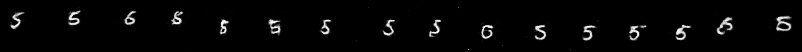
\includegraphics[width=0.8\linewidth]{../progress/imgs/mnist/mode_collapse2.png}
    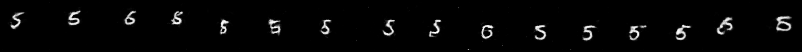
\includegraphics[width=0.8\linewidth]{../progress/imgs/mnist/mode_collapse3.png}
\end{figure}

\begin{figure}[H]\label{fig:wrongdir_base}
    \centering
    \caption{Video for the text `the digit 9 is moving down and up' (real is top, generated is bottom)}
    
\includegraphics[width=0.8\linewidth]{../progress/imgs/mnist/minst_9_true.png}\\
    
\includegraphics[width=0.8\linewidth]{../progress/imgs/mnist/minst_fake_9.png}
\end{figure}


\subsubsection{My Method}
My method produces pretty high quality examples, with little to no digit morphing. It should also be noted that little mode collapse was observed as well. However, as it can be clearly seen, little to no care about the sentence is made, suggesting the loss for conditioning is not being prioritised.

\begin{figure}[H] \label{fig:my_no_corr}
    \centering
    \caption{From top to bottom: `$<$start$>$ digit 9 is left and right$<$end$>$', `$<$start$>$ digit 8 is right and left$<$end$>$' `$<$start$>$ digit 8 is bottom and top$<$end$>$' and `$<$start$>$ digit 4 is top and bottom$<$end$>$'}
    
\includegraphics[width=0.8\linewidth]{images/cond_mnist/1.jpg}\\
    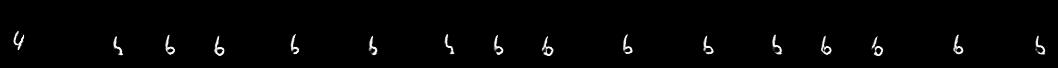
\includegraphics[width=0.8\linewidth]{images/cond_mnist/2.jpg}\\
    
\includegraphics[width=0.8\linewidth]{images/cond_mnist/3.jpg}\\
    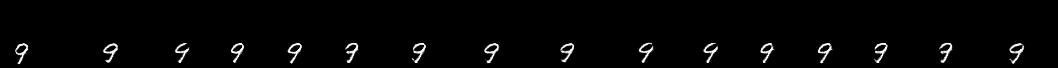
\includegraphics[width=0.8\linewidth]{images/cond_mnist/4.jpg}\\
\end{figure}

\subsection{MRVDC}

\subsubsection{TCWYT Baseline}

\begin{figure}[H]
    \centering
    \caption{Good visual results from two different videos (sampled from the training set).}
    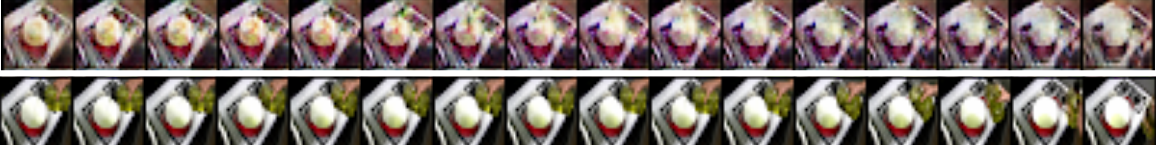
\includegraphics[width=0.8\linewidth]{../progress/imgs/mrvdc/good_1.png}\\
    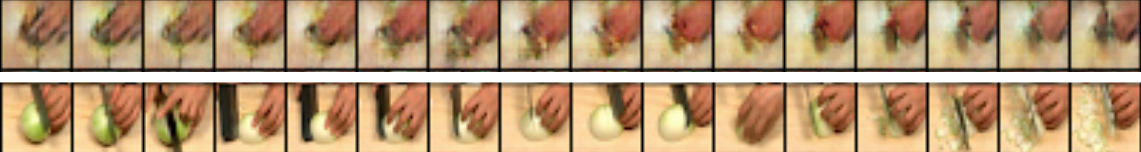
\includegraphics[width=0.8\linewidth]{../progress/imgs/mrvdc/good_2.png}
\end{figure}

\begin{figure}[H]
    \centering
    \caption{Bad quality videos sampled from the training process.}
    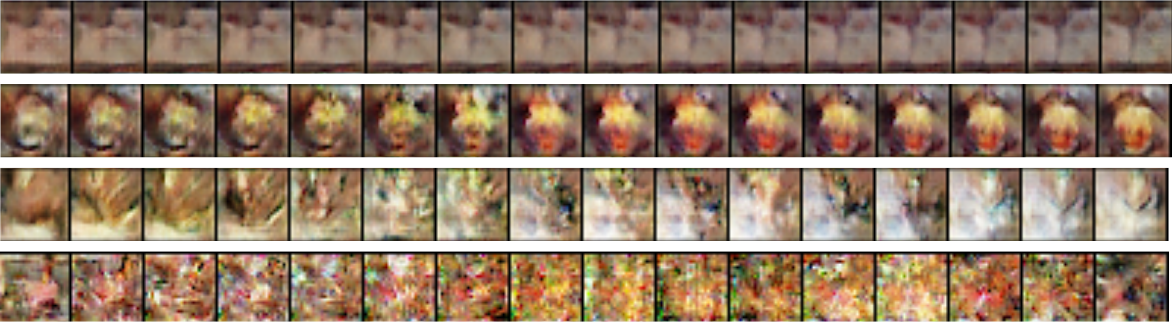
\includegraphics[width=0.8\linewidth]{../progress/imgs/mrvdc/bad_quality.png}
\end{figure}

\begin{figure}[H]
    \centering
    \caption{Three samples from the testing set with the ground truth on the bottom. For the sentence (tokenized): `$<$start$>$ a woman is saying about how to make vegetable tofu $<$unk$>$ $<$end$>$'}
    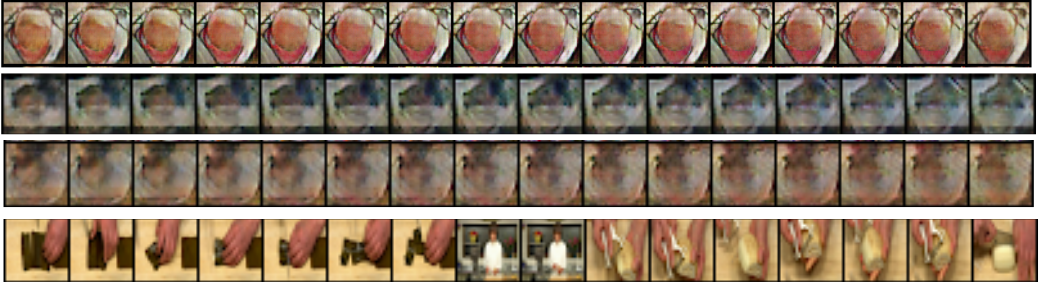
\includegraphics[width=0.8\linewidth]{../progress/imgs/mrvdc/test1.png}
\end{figure}

\begin{figure}[H]
    \centering
    \caption{Three samples from the testing set with the ground truth on the bottom. For the sentence (tokenized): `$<$start$>$ the person is cooking $<$end$>$'}
    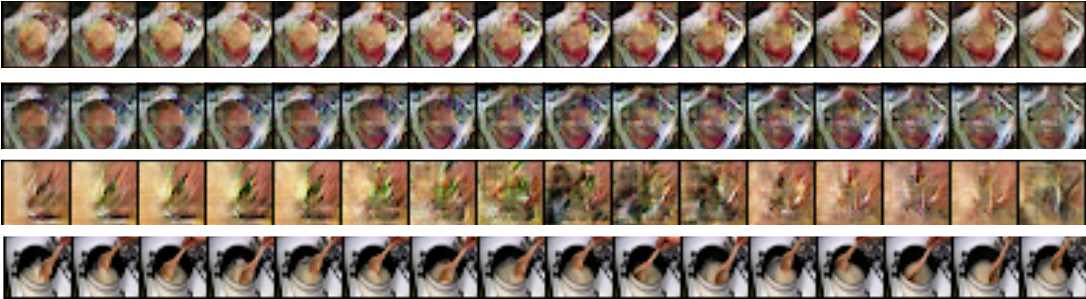
\includegraphics[width=0.8\linewidth]{../progress/imgs/mrvdc/test2.png}
\end{figure}

\subsubsection{TGANv2 Baseline}

Overall, this model does pretty well, but there are still signs of mode collapse (as seen in the 4th and 5th row of Figure \ref{fig:uncond_mr}), and it is clear that some overfitting is performed due to . The last row suggests that the discriminator does not respect motion as much as I hypothesised it would. Some poor examples are shown in Figure \label{fig:uncond_bad}.

\begin{figure}[H]
    \label{fig:uncond_mr}
    \centering
    \caption{Various generated samples from MRVDC with a re-implementation of TGANv2 (rescaled from 128x128 to fill the line). }
    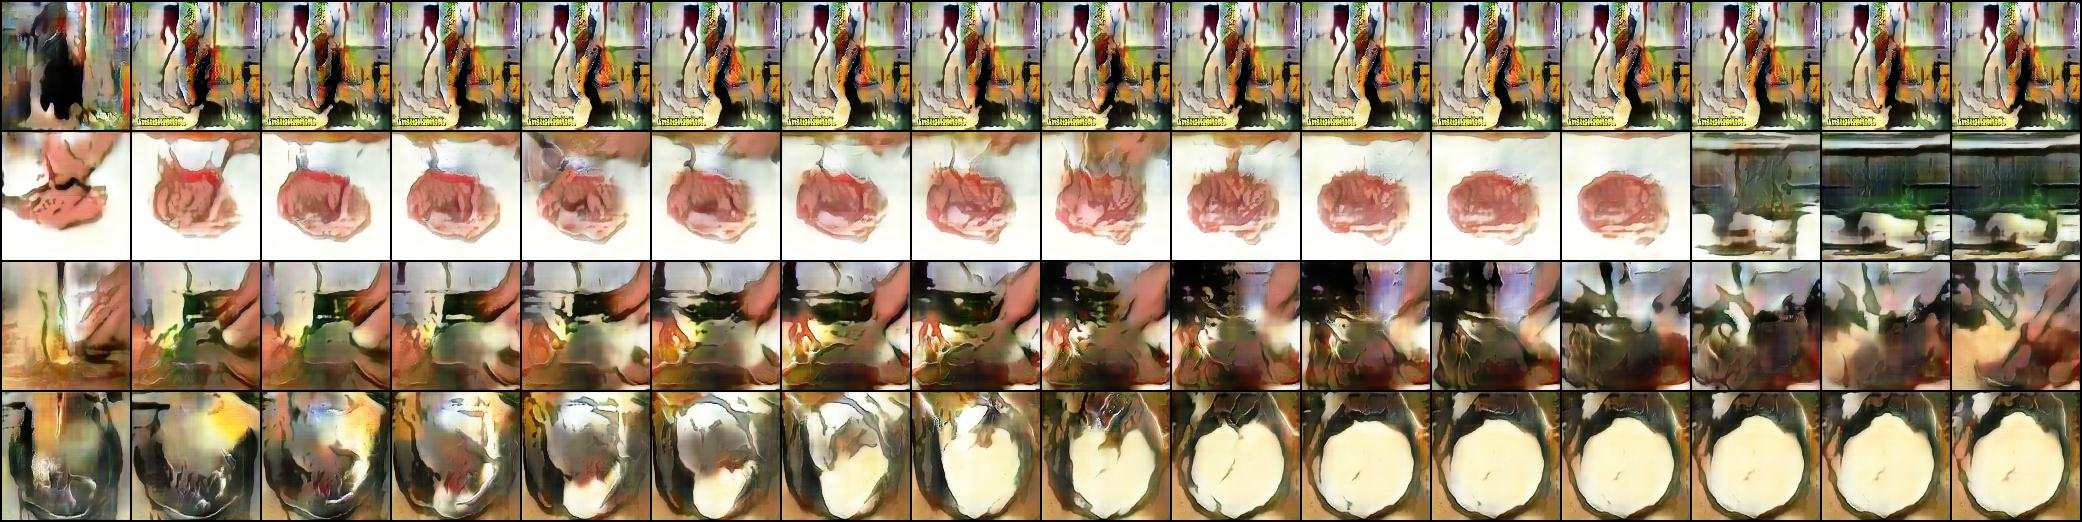
\includegraphics[width=0.95\linewidth]{images/uncond_mr/1.jpg}\\
    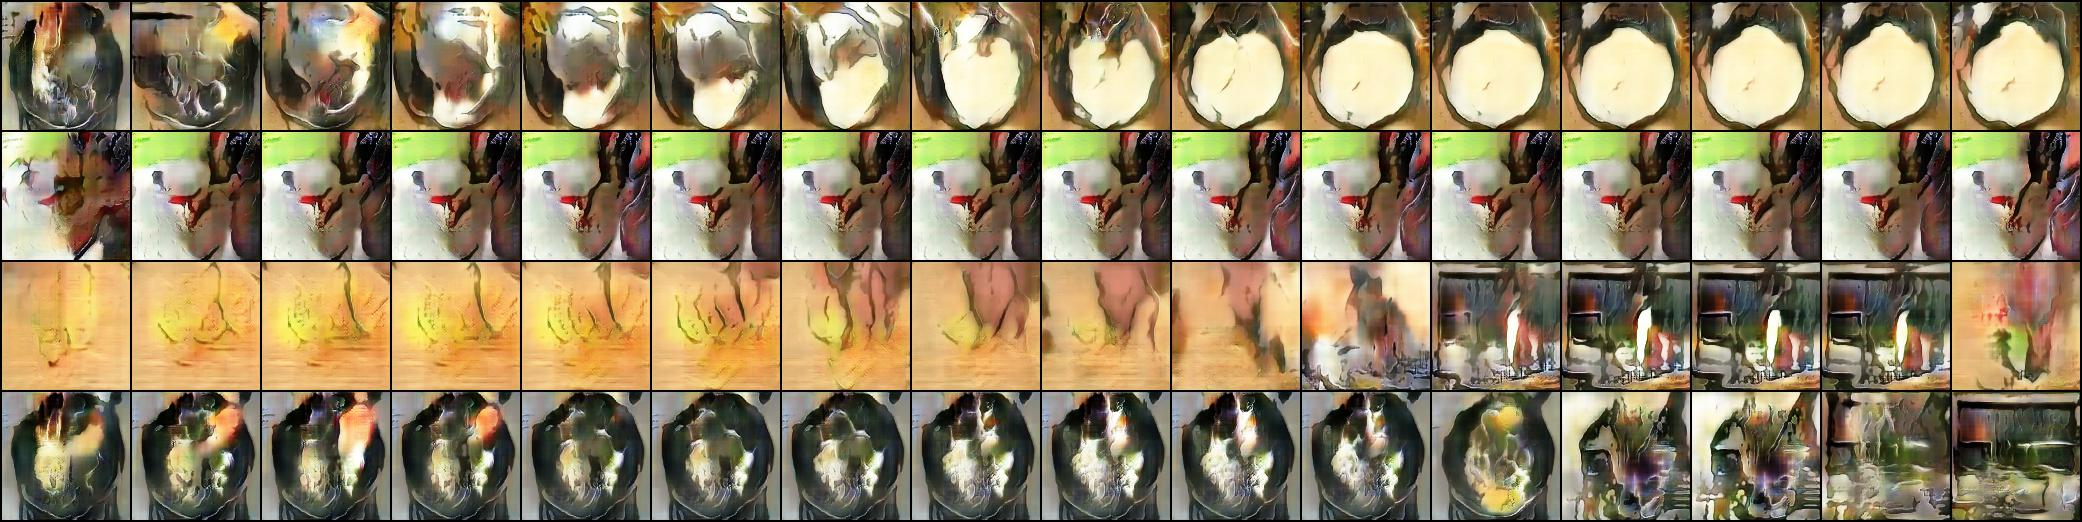
\includegraphics[width=0.95\linewidth]{images/uncond_mr/2.jpg}\\
    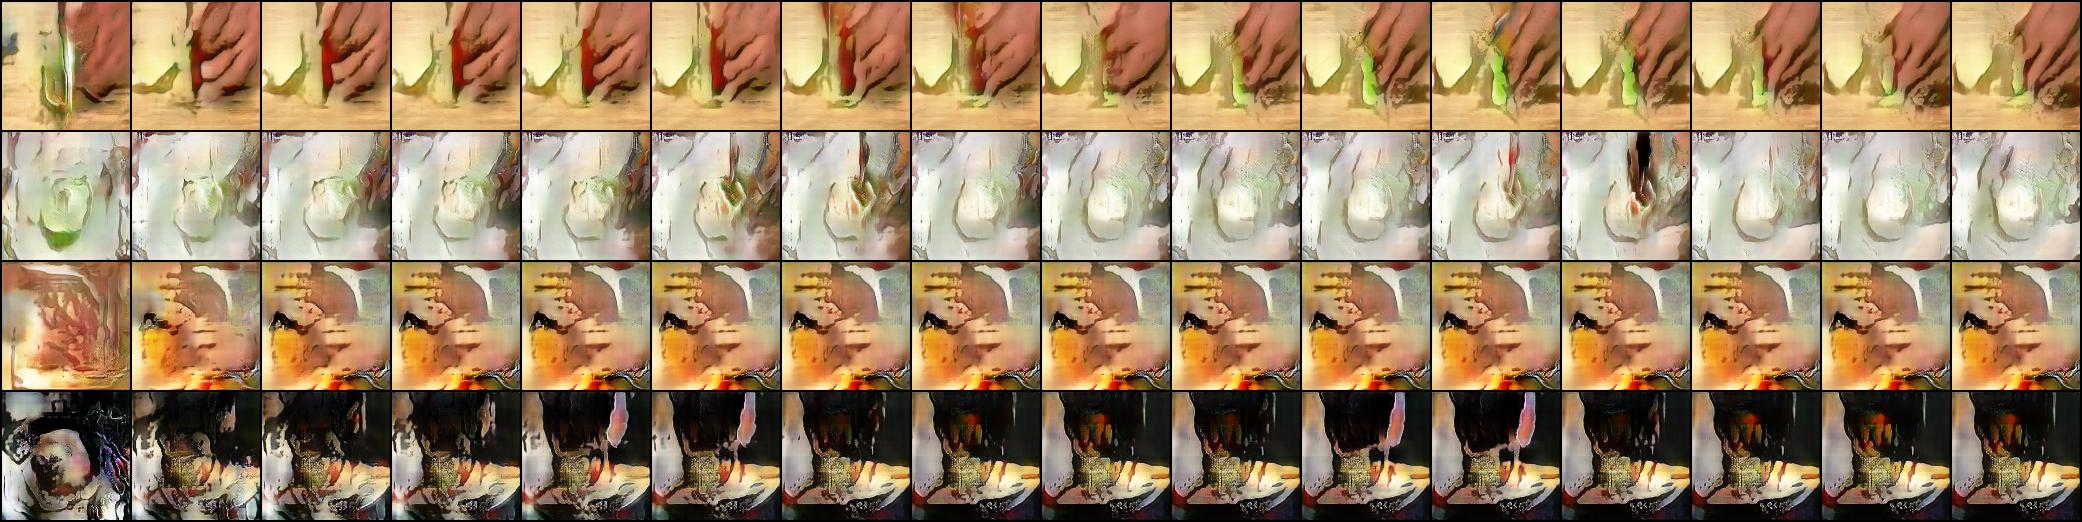
\includegraphics[width=0.95\linewidth]{images/uncond_mr/3.jpg}
\end{figure}

\begin{figure}[H]
    \label{fig:uncond_mr}
    \centering
    \caption{Some poorly generated samples from MRVDC from a training batch. }
    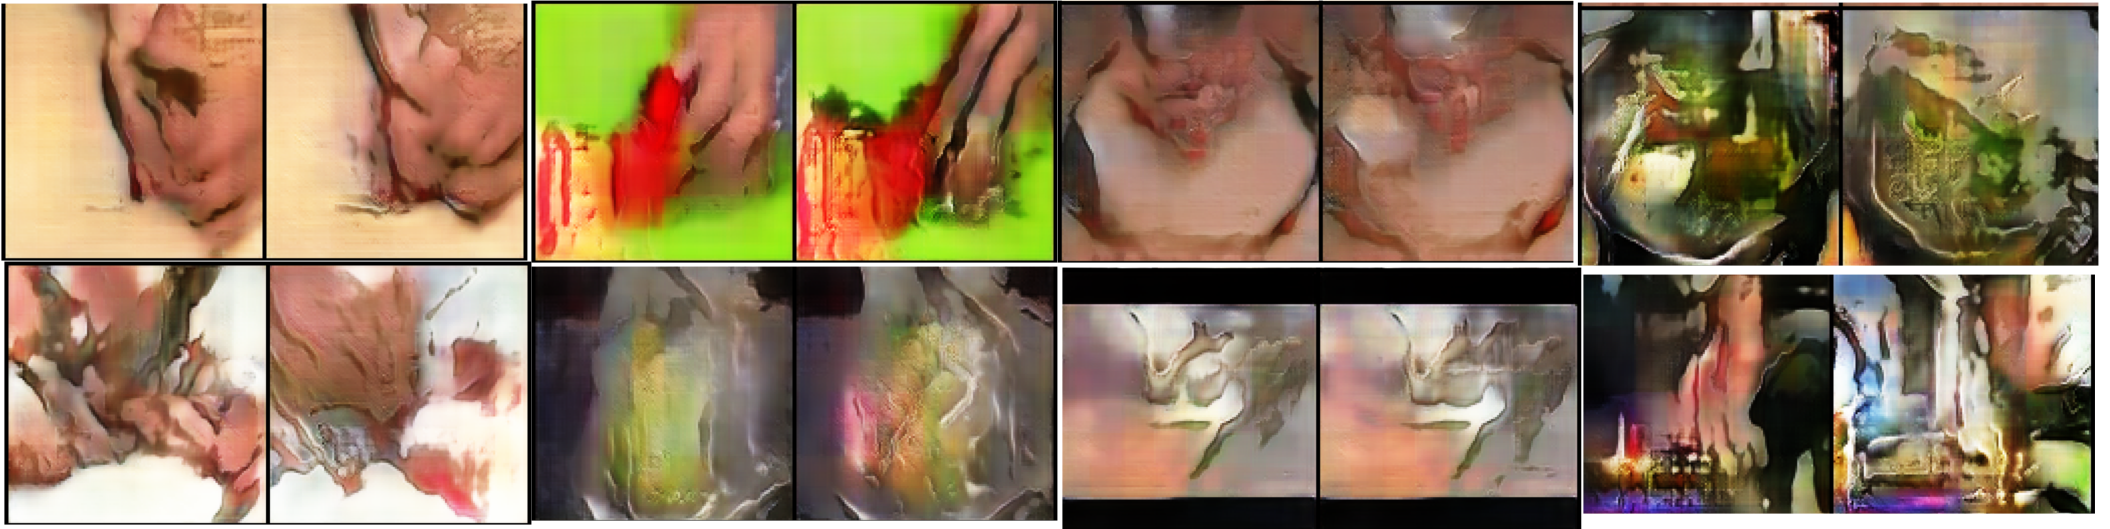
\includegraphics[width=0.8\linewidth]{images/unconditional_bad.png}
\end{figure}

I would argue my implementation is near-perfect. Further testing on UCF-101 \cite{noauthor_ucf101_nodate} is required to be done with a larger number of iterations performed in order to be certain.

\subsubsection{My Method}

It is clear that the samples produced are not of as high quality as the unconditional case. I believe this is due to either using a smaller resolution video, smaller batch size and/or the suggested combination of conditional and unconditional loss. All three variables were played with on a K80 on Adelaide Uni Phoenix HPC. But as mentioned, every attempt to train this model with a higher resolution on a K80 (rather than V100), but did not succeed in finding a set of parameters where the GAN did not instantly diverge it's discriminator and/or generator loss. Further experimentation is required.

These results also suggest that sentences again are not really cared for.

\begin{figure}[H]
    \label{fig:cond_mr}
    \centering
    \caption{Generated samples from the conditional model and their real associated video. From top to bottom: `$<$start$>$ the man poured preserves over the chicken$<$end$>$', `$<$start$>$ a person is dicing and onion$<$end$>$', `$<$start$>$ a woman is peeling a large shrimp in a glass bowl of water$<$end$>$'}
    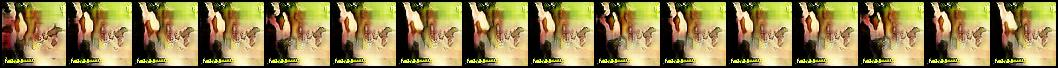
\includegraphics[width=0.95\linewidth]{images/cond_mr/1.jpg}\\
    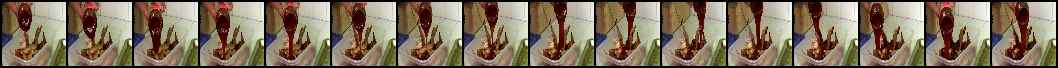
\includegraphics[width=0.95\linewidth]{images/cond_mr/1.png}\\
    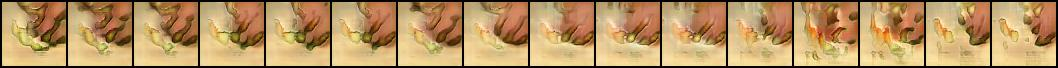
\includegraphics[width=0.95\linewidth]{images/cond_mr/2.jpg}\\
    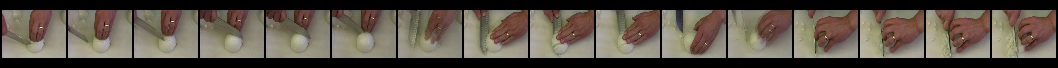
\includegraphics[width=0.95\linewidth]{images/cond_mr/2.png}\\
    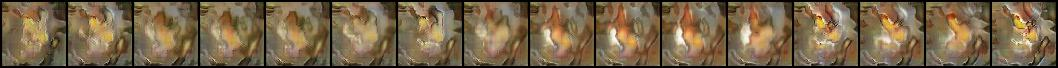
\includegraphics[width=0.95\linewidth]{images/cond_mr/3.jpg}\\
    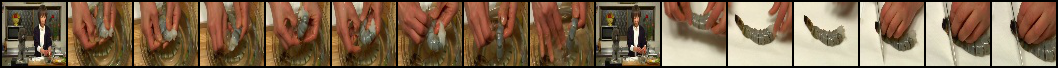
\includegraphics[width=0.95\linewidth]{images/cond_mr/3.png}\\
\end{figure}

\subsection{Observations During Training}

\begin{enumerate}
    \item Larger batch sizes seems to helps with quality and producing reasonable looking samples faster, further supporting the findings in \cite{brock_large_2018,saito_tganv2:_2018}
    \item Model is very sensitive to hyper-parameters. Even running the same model with the same hyper-parameters (and version of PyTorch, 1.1.0) on a K80 (on University of Adelaide's Phoenix HPC) verses locally with a GTX 1060, causes the model to diverge. An example of what occurs to the produced samples due to this sensitivity is shown in Figure \ref{fig:wtf_samples}. This is either due to a different implementation of cuDNN or some bug in my code.
    \item Utilising WGAN-GP \cite{heusel_gans_2017} did not help. When WGAN-GP \cite{heusel_gans_2017} was utilised, 5 discriminator steps was required to produce reasonable results.
    \item When WGAN \cite{arjovsky_wasserstein_2017} was experimented with, I could not find a set of parameters that would train the TCWYT baseline model.
    \item Batch normalization \cite{ioffe_batch_2015} is important for the TCWYT \cite{pan_create_2018} model, without it, horrible results would be produced.
    \item Zero-centred gradient penalty \cite{saito_tganv2:_2018} helped significantly during the training of the unconditional and conditional model, contrary to what \cite{saito_tganv2:_2018} claimed. This is possibly due to some differences in my implementation, larger resolution models being trained in TGANv2 or a different (and smaller) dataset begin trained on.
\end{enumerate}

\begin{figure}[H] \label{fig:wtf_samples}
    \centering
    \caption{When the equivalent model with the same hyper-parameters is trained on a K80 on Adelaide Uni Phoenix HPC}
    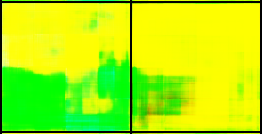
\includegraphics[width=0.4\linewidth]{images/wtf_1.png}\\
    
\includegraphics[width=0.8\linewidth]{images/wtf_2.png}\\
\end{figure}


\blankpage
\chapter{Conclusion}

To conclude, this thesis covered many concepts related to generative modelling and GANs. The state of the art research was covered and discussed in-depth. An implementation of two baseline models were made, which can be utilised for future development purposes, namely TCWYT \cite{pan_create_2018} and TGANv2 \cite{saito_temporal_2016} (both papers did not release code). Finally, modifications of TGANv2 were made to support conditioning information. Most notably, it was found that the text encoding was not cared about during generation of moving MNIST. The current results in the conditional case for cooking clips in MRVDC are of poor quality compared to the unconditional counter-part, this is likely due to the smaller batch size and smaller video resolution used when training. Further experimentation is required.

\section{Future Work}
Quite a lot can be improved on, most notably:

\begin{enumerate}
    \item Utilising GPT-2 as a text encoding method to see how significant the sentences are on the production of models.
    \item Improving my experimental setup, with quantitative metrics to measure video quality and sentence correlation to produced videos. Even a simple score such as a FID or Inception Score would be better than the current subjective method of evaluation.
    \item Utilising better datasets, where some are restricted to a certain domain. Restricting the domain seems to produce the best results in many papers. 
    \item Improving the speed of my current implementation, as training with a larger number of iterations seems to likely benefit the sample generation, e.g. with 100k iterations.
    \item Modifying the implementation to use FP16 or mixed precision training, to speed training up. Many existing state of the art architectures (e.g. BigGAN) utilise mixed precision training, so it should be possible.
    \item Modifying the generator to be more similar to BigGAN, e.g. by using BigGAN-deep
    \item Ensuring my implementation of TGANv2 is as good as the paper's results, I suspect is it, but the only way to test would be to train my implementation on UCF-101 \cite{noauthor_ucf101_nodate}.
\end{enumerate}

\bibliography{Thesis}
\bibliographystyle{plain}

\end{document}

